\section{研究课题论证}

\subsection{深度学习模型与大数据}

\begin{xframe}{Big Data \& Deep Learning}

    \begin{columns}
        \column{0.5\textwidth}<1->
        \begin{itemize}
            \item {Data\\
            \descriptionstyle{物联网与信息存储技术的革新带来更大更丰富的数据}}
            \item {Idea\\
            \descriptionstyle{海量数据与实验启发着研究人员的灵感}}
            \item {Code\\
            \descriptionstyle{既有的深度学习框架帮助研究人员快速构建深度神经网络}
            }
            \item {Experiment\\
            \descriptionstyle{CUDA框架与新的网络训练方式极大提高了实验速度}
            }
        \end{itemize}
        \column{0.6\textwidth}<1->
            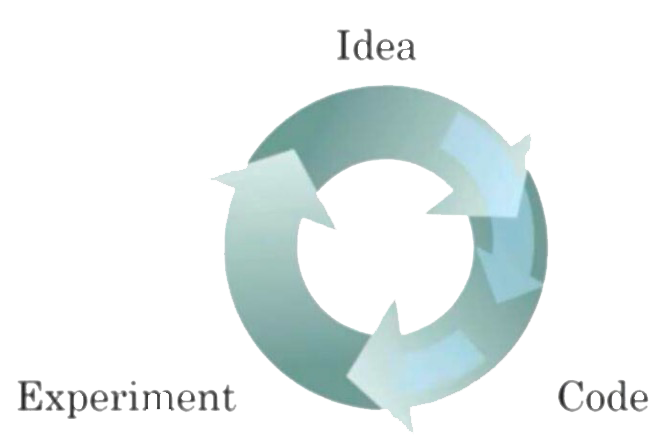
\includegraphics[width=\textwidth,totalheight=0.5\textheight]{./style/images/circle.png}

    \end{columns}

\end{xframe}


\subsection{时间序列数据}

\begin{xframe}{Time Series Data}

    \begin{itemize}
        \item {\descriptionstyle{大数据的背景}:\\
        \descriptionstyle{时间序列数据亦具备规模巨大(如:电力负荷)、模态多样(如:流媒体)和关联复杂(如:股票油价)的性质}}
        \item {\descriptionstyle{时序数据的难题}:\\
        \descriptionstyle{作为一种动态机制不确定的数据,如何建立一种可逼近的学习模型来克服大规模时间序列数据非平稳状态下的动态性逼近或分类问题}}
    \end{itemize}

    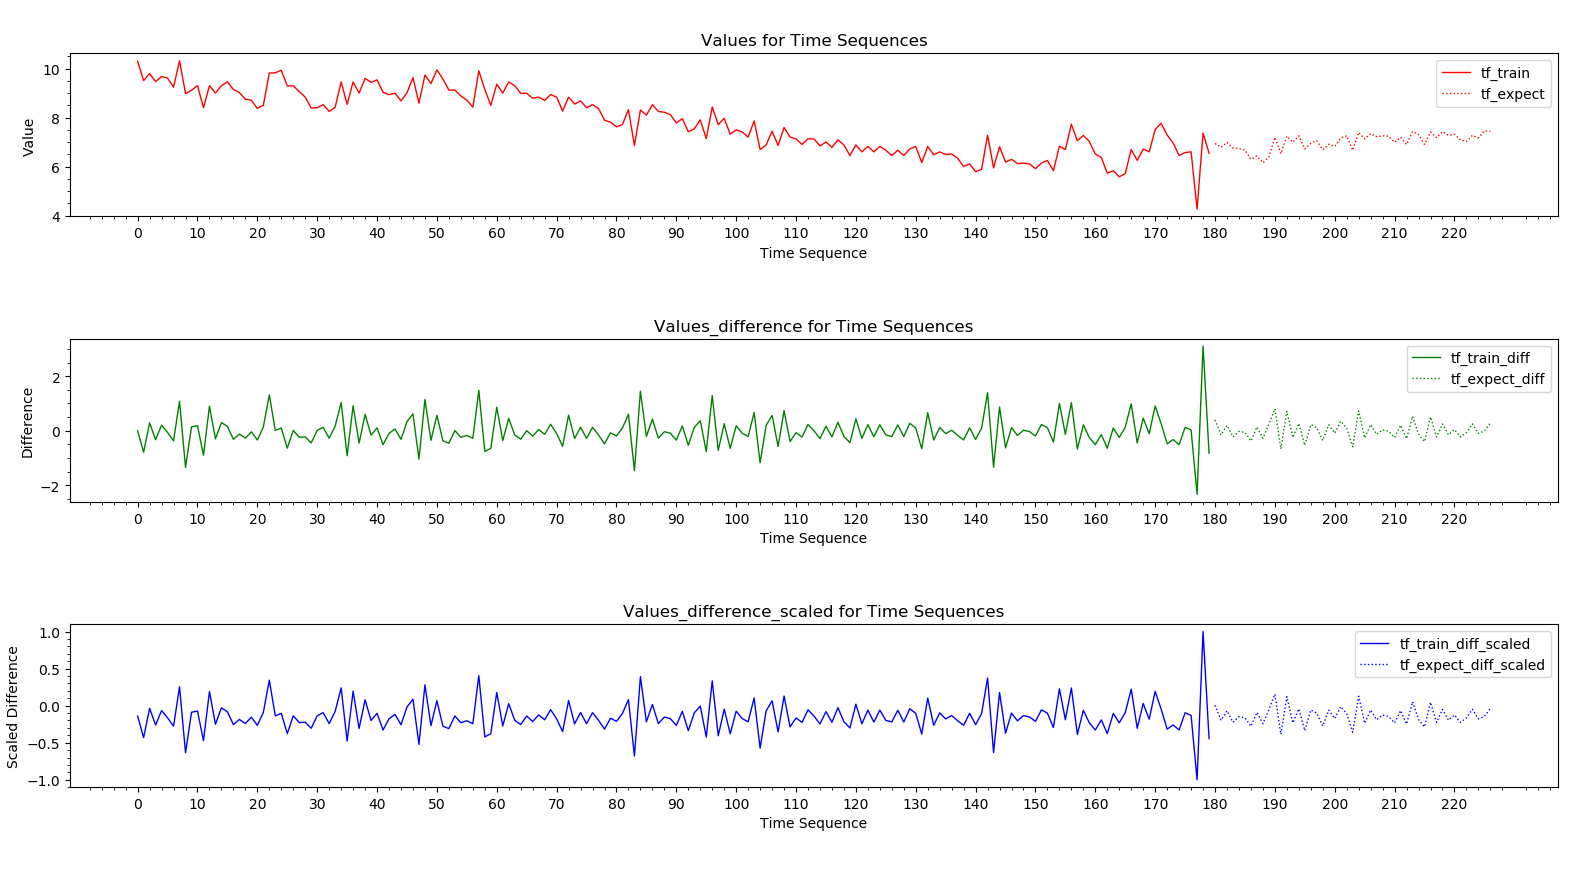
\includegraphics[width=\textwidth,totalheight=0.5\textheight]{./style/images/tf3.png}

\end{xframe}

\subsection{RNN}

\begin{xframe}{Recurrent NN}

    \begin{columns}
        \column{0.5\textwidth}<1->
        \begin{itemize}
            \item {ANN\\
            \descriptionstyle{将输入同时前向传播至隐藏层,未体现序列性质}}

            \vspace{3em}

            \item {RNN\\
            \descriptionstyle{将输入按序列输入至隐藏层,当前隐藏层的状态受当前输入与上一隐藏层状态的共同影响}}
        \end{itemize}
        \column{0.5\textwidth}<1->
        \begin{center}
            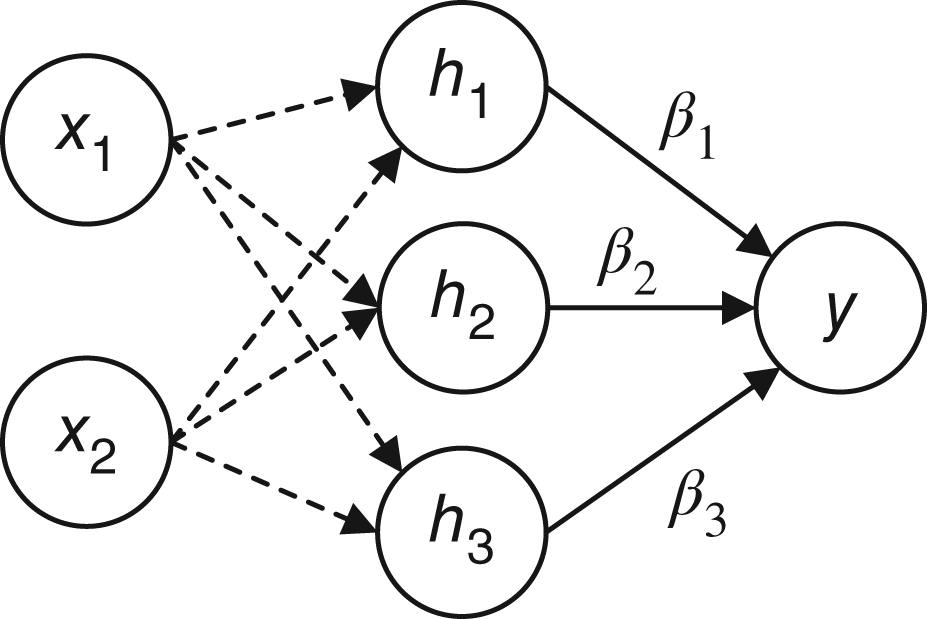
\includegraphics[height=0.3\textheight]{./style/images/fc.png}

            ANN

            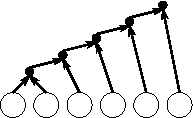
\includegraphics[height=0.3\textheight]{./style/images/rnn.pdf}

            RNN
        \end{center}

    \end{columns}
\end{xframe}

\begin{xframe}{Recurrent NN}

    \begin{itemize}
        \item {\descriptionstyle{RNN的展开}}
    \end{itemize}

    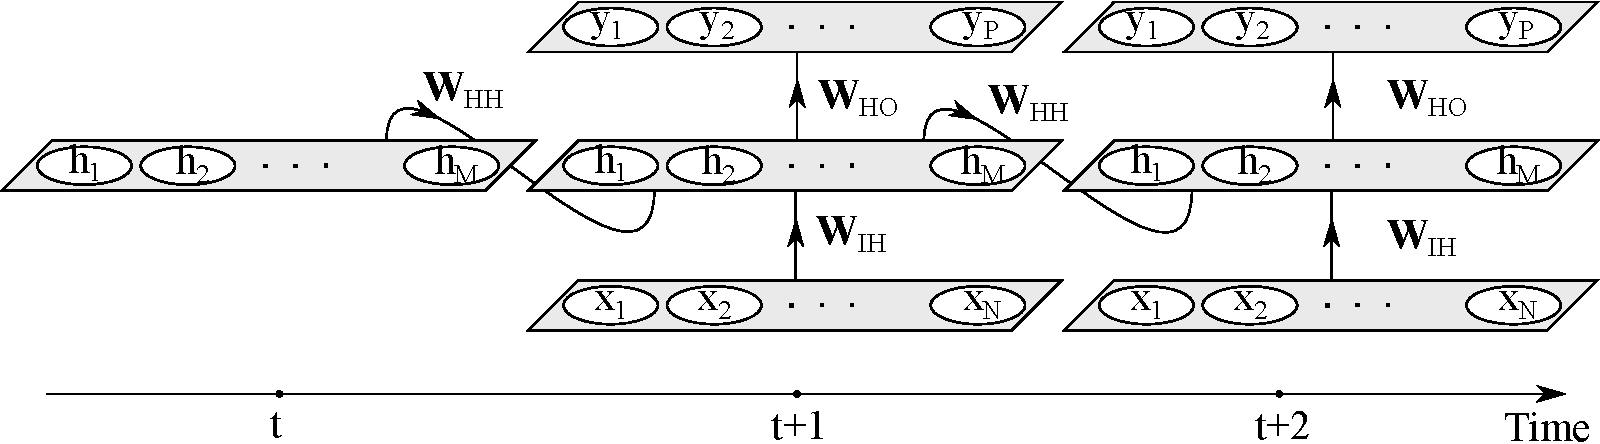
\includegraphics[width=\textwidth,totalheight=0.5\textheight]{./style/images/srnn.pdf}

\end{xframe}

\begin{xframe}{Recurrent NN}

    \begin{itemize}
        \item {\descriptionstyle{RNN的应用问题}:\\
        \descriptionstyle{在将长序列作为输入时,因为激活函数的特性,RNN的训练有可能会出现梯度消失或者梯度爆炸的现象}}
    \end{itemize}


    \begin{columns}
        \column{0.5\textwidth}<1->
        \begin{center}
            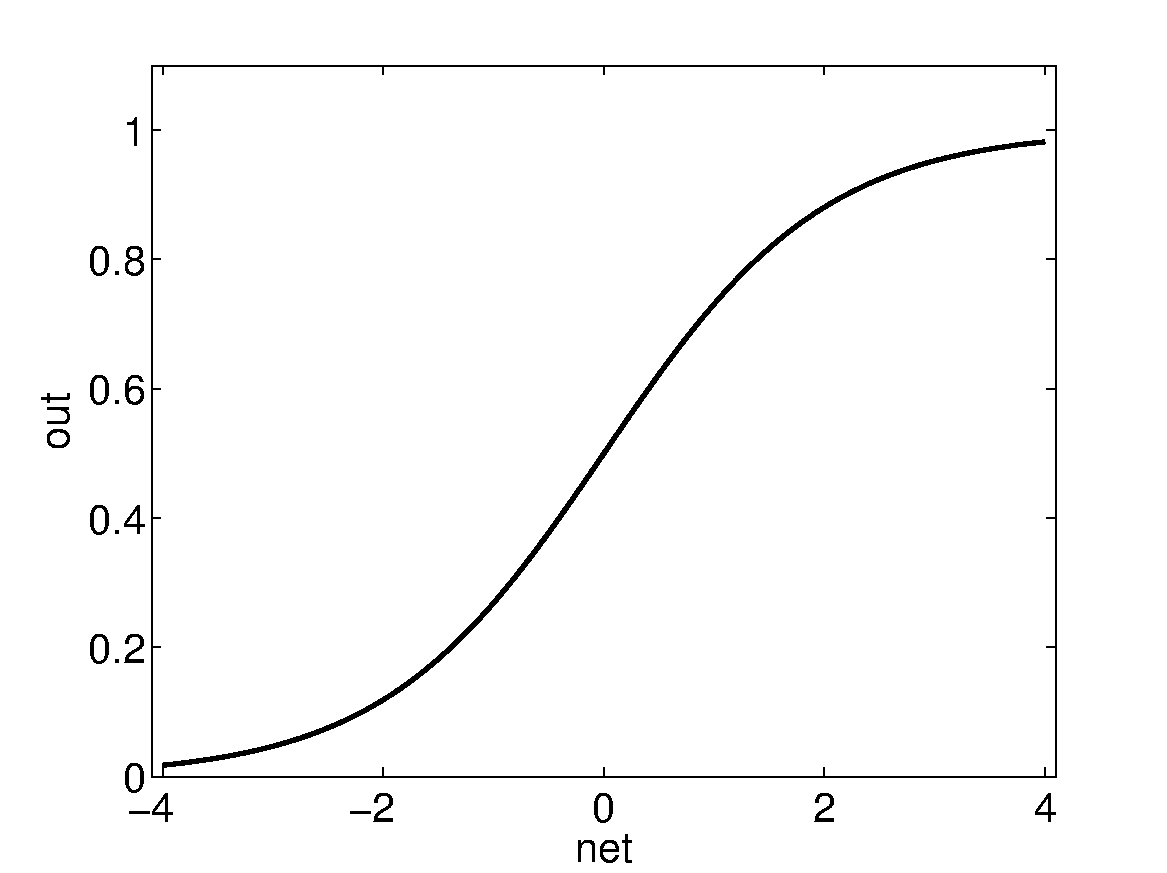
\includegraphics[width=\textwidth,height=0.5\textheight]{./style/images/logistic.pdf}
            Sigmod
        \end{center}

        \column{0.5\textwidth}<1->
        \begin{center}
            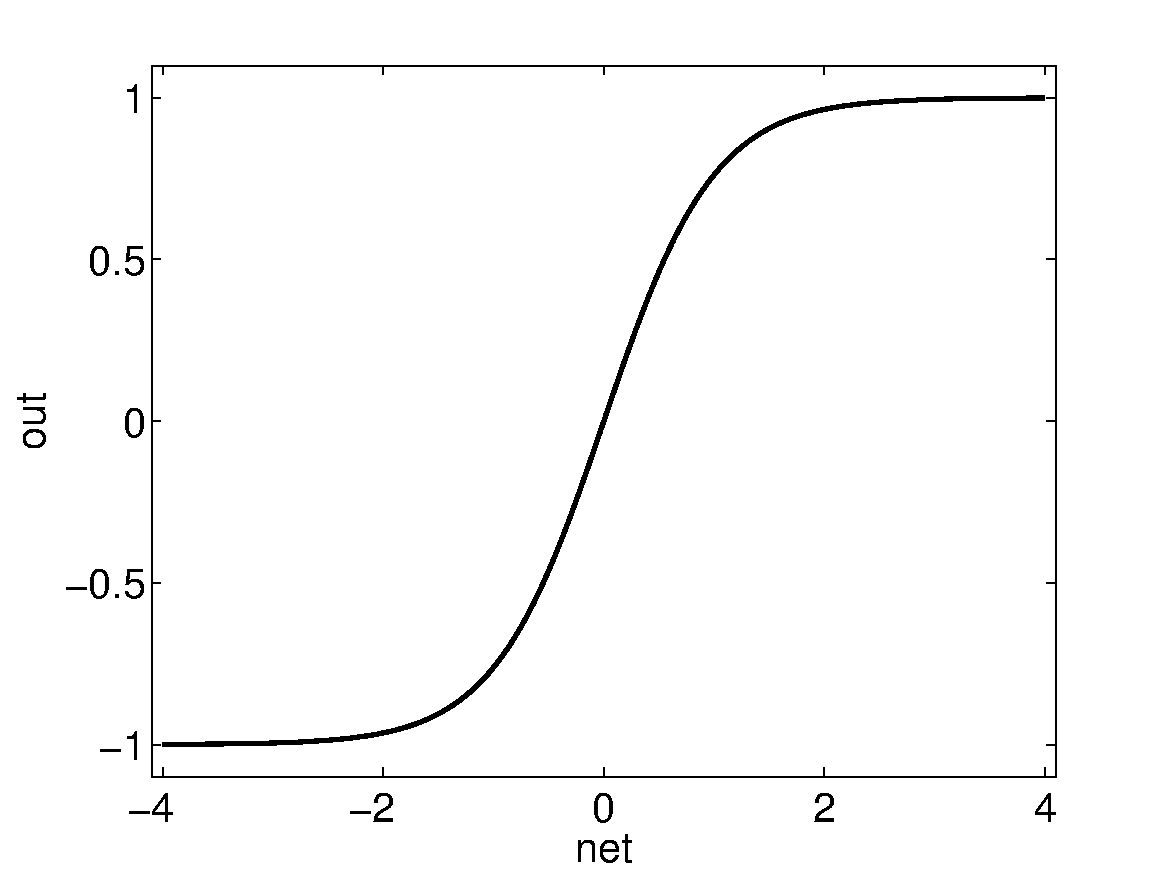
\includegraphics[width=\textwidth,height=0.5\textheight]{./style/images/tanh.pdf}
            Tanh
        \end{center}

    \end{columns}

\end{xframe}

\begin{xframe}{LSTM \& GRU}


    \begin{columns}
        \column{0.5\textwidth}<1->
        \begin{center}
            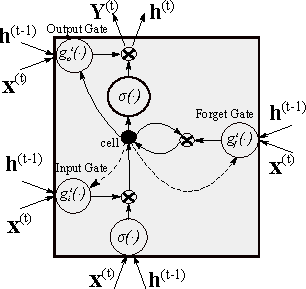
\includegraphics[width=\textwidth]{./style/images/LSTM_cell.pdf}
            
        \end{center}

        \column{0.5\textwidth}<1->
        \begin{center}
            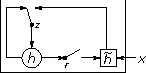
\includegraphics[width=\textwidth]{./style/images/gru.pdf}
        \end{center}

    \end{columns}

    \begin{columns}
        \column{0.5\textwidth}<1->
        \begin{center}
            LSTM
        \end{center}

        \column{0.5\textwidth}<1->
        \begin{center}
            GRU
        \end{center}

    \end{columns}

\end{xframe}

\begin{xframe}{Train Example}
    
    \includemedia[
        % label=train,
        width=1.0\linewidth,
        height=0.275\linewidth, % 16:9
        addresource=train.mp4, 
        transparent,
        activate=pagevisible,
        % deactivate=pageinvisible,
        % passcontext,
        flashvars={
        source=train.mp4
        &scaleMode=stretch
        &autoPlay=true % start playing on activation
        &loop=true
        &hideBar=true
        }
      ]{}{VPlayer.swf}

\end{xframe}
